\chapter{Remote graphical applications}

% This chapter explains how to start graphical applications on a remote computer, such that you can interact with its graphical interface locally.


Up to this point, we've issued commands through the terminal.  The terminal is a powerful tool, but sometimes it's also useful to run graphical programs\index{graphical programs} (as opposed to text-based terminal programs) remotely, for example when you want to use the graphical debugging capabilities that the MATLAB GUI offers to debug some of your code on LISA. Within the context of optimization, another typical application of running graphical applications remotely is that you can have the LISA system generate figures showing the progress of the optimization similar to the one in Fig.~\ref{fig:plotseq-1-600}, which you can then view and manipulate (e.g.~zoom, pan) from your local machine. Amazingly, this is possible through a process called \textit{X forwarding over SSH}\index{X!forwarding over SSH}. Here, `X'\index{X} refers to the program that takes care of visualization on Linux. The Linux operating system is telling X what to visualize, and then X figures out which pixels on what screen should be what color, and whether a particular pixel is part of, say, a button, drop-down list, or some other user interface element. It is possible to re-route messages to the X system through your SSH connection, such that they end up on your local machine. If your local system is Linux, the X messages that your system receives can be interpreted by your local copy of the X program, and the user interface of graphical application that is running on the remote machine will be displayed locally. However, you are probably running Windows, so you need to install a Windows version of X first. 

Download Xming\index{Xming} from \burl{http://sourceforge.net/projects/xming/files/Xming/6.9.0.31/Xming-6-9-0-31-setup.exe/download} and install it. Now go to the Windows start menu and click XLaunch (Fig.~\ref{fig:xlaunch-0}). This will bring up a wizard (Fig.~\ref{fig:xlaunch-1}). Follow the steps outlined in Figs.~\ref{fig:xlaunch-2}--\ref{fig:xlaunch-4}. 

\begin{figure}[H]
  \centering
    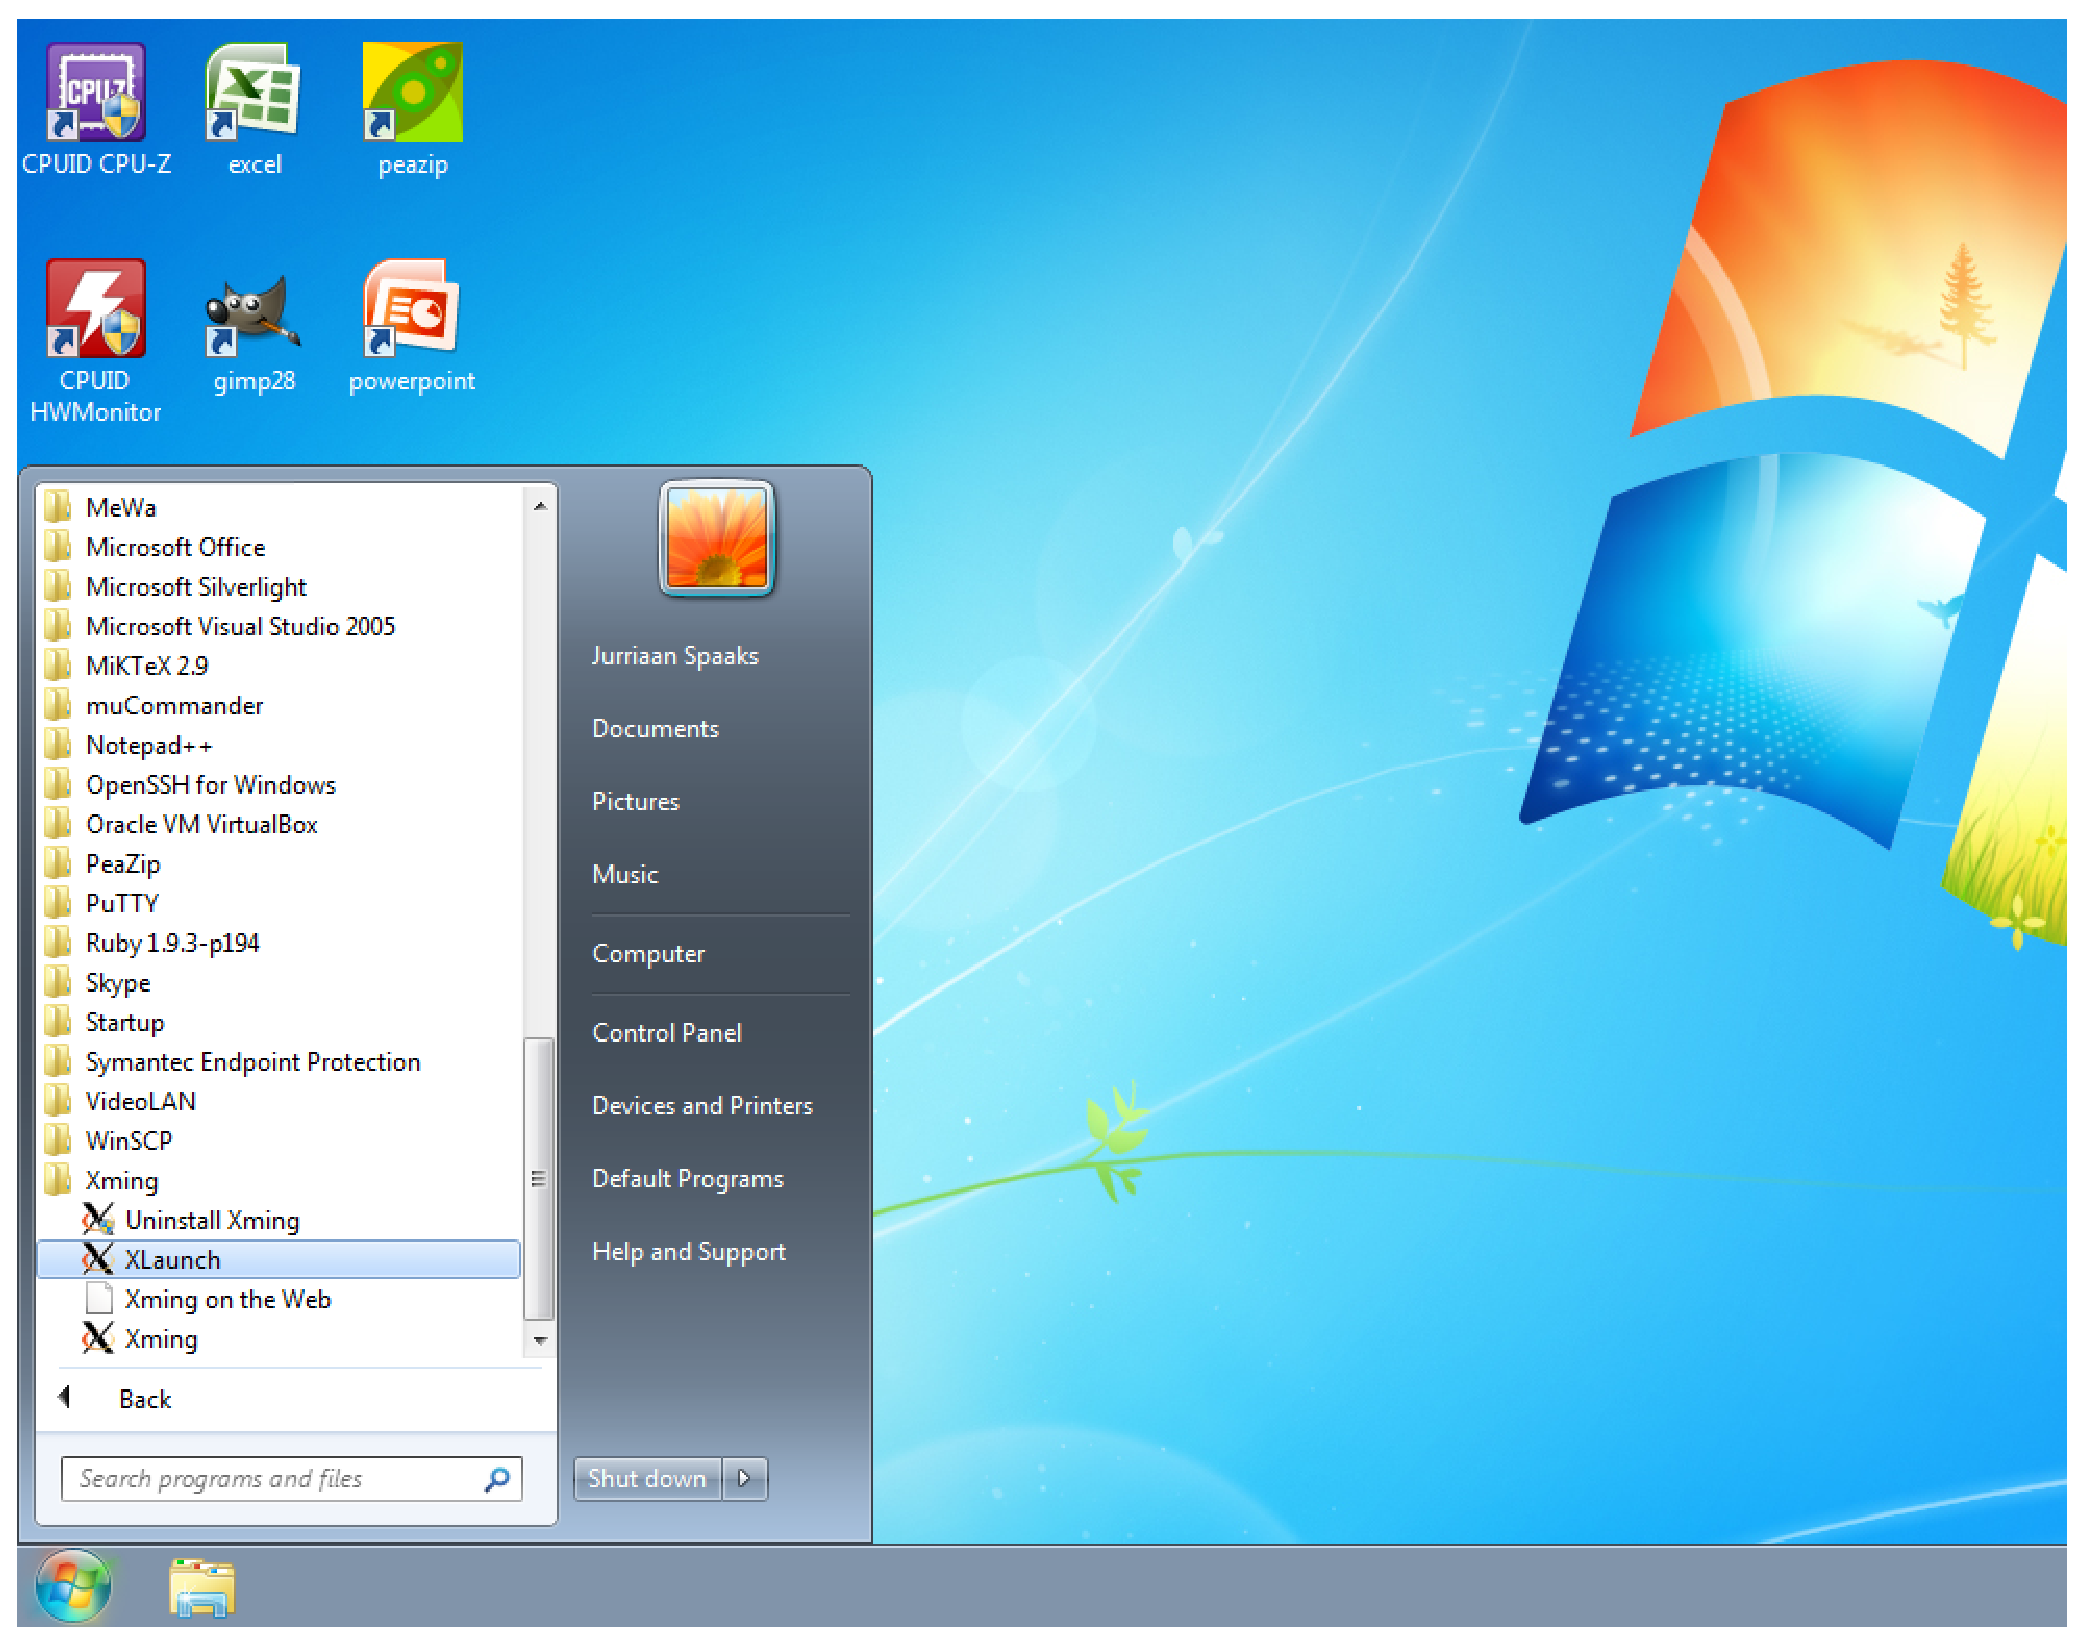
\includegraphics[width=0.8\textwidth]{./../eps/xlaunch-1.eps}
  \caption{Starting XLaunch from the Windows 7 start menu.}
  \label{fig:xlaunch-0}
\end{figure}


\begin{figure}[H]
  \centering
    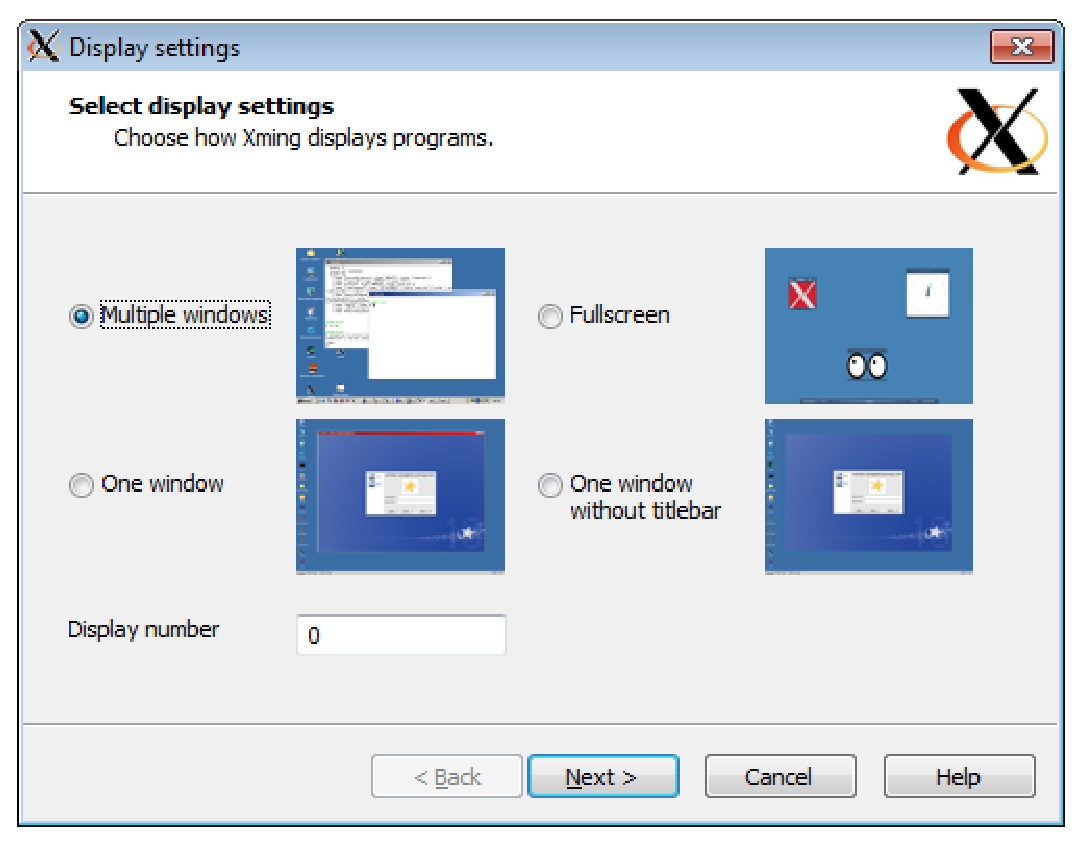
\includegraphics[width=0.7\textwidth]{./../eps/xlaunch-2.eps}
  \caption{The XLaunch configuration wizard page 1.}
  \label{fig:xlaunch-1}
\end{figure}

\begin{figure}[H]
  \centering
    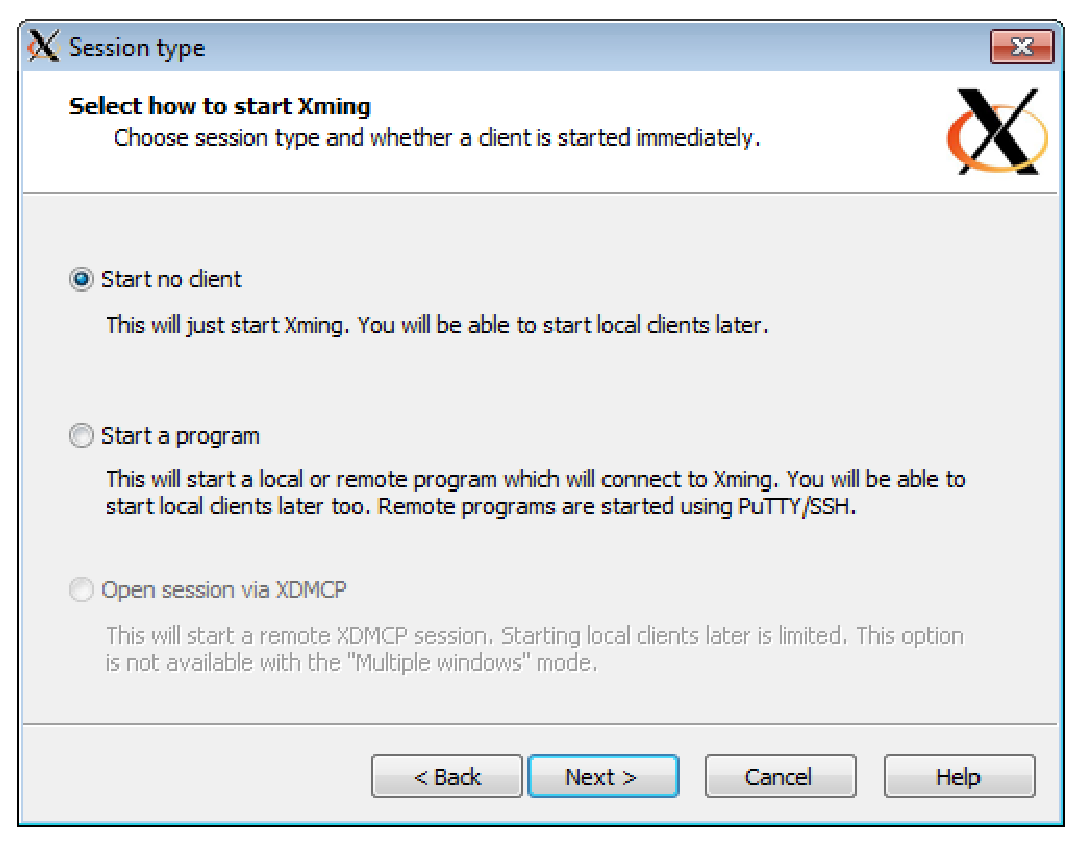
\includegraphics[width=0.7\textwidth]{./../eps/xlaunch-3.eps}
  \caption{The XLaunch configuration wizard page 2.}
  \label{fig:xlaunch-2}
\end{figure}

\begin{figure}[H]
  \centering
    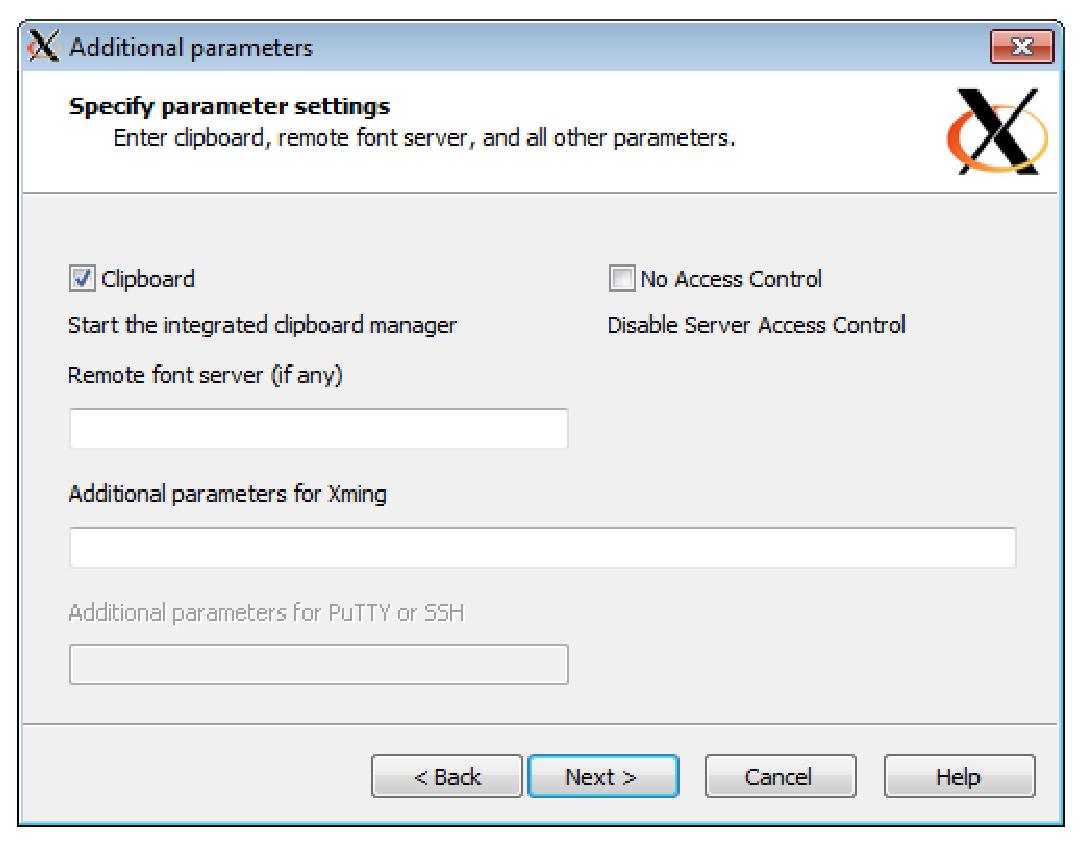
\includegraphics[width=0.7\textwidth]{./../eps/xlaunch-4.eps}
  \caption{The XLaunch configuration wizard page 3.}
  \label{fig:xlaunch-3}
\end{figure}

\begin{figure}[H]
  \centering
    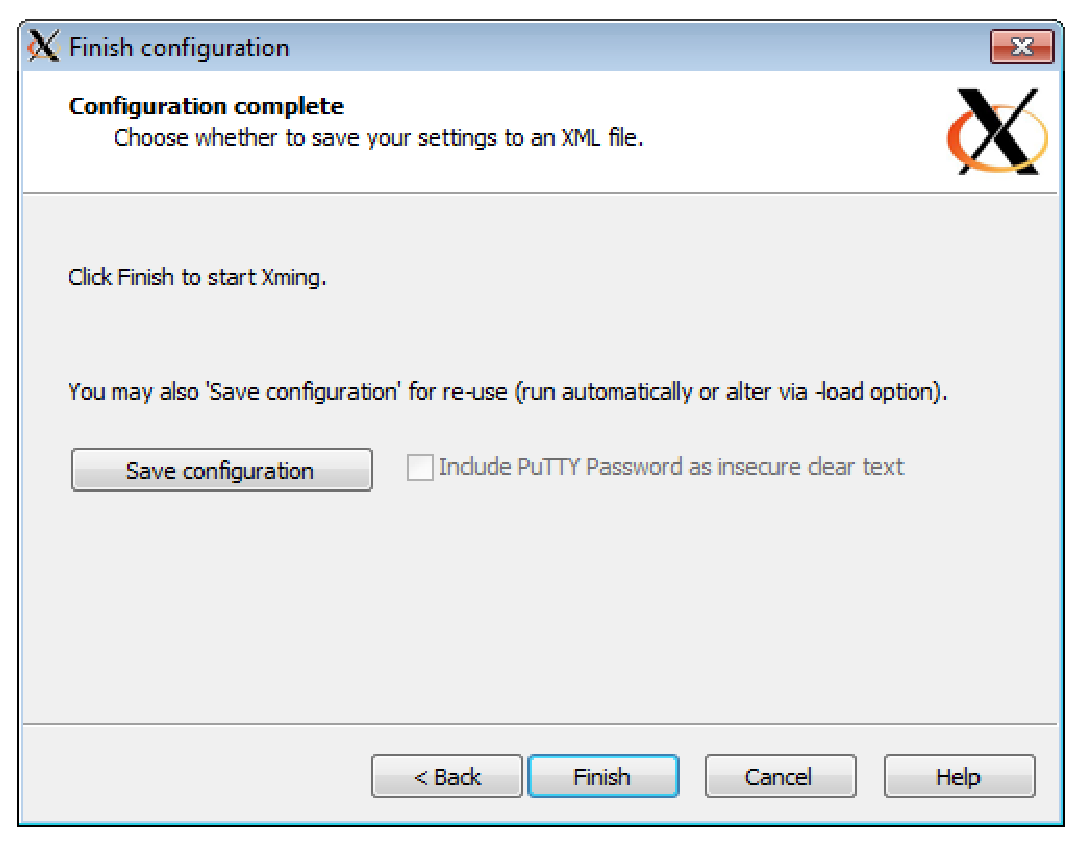
\includegraphics[width=0.7\textwidth]{./../eps/xlaunch-5.eps}
  \caption{The XLaunch configuration wizard page 4.}
  \label{fig:xlaunch-4}
\end{figure}



After you go through the XLaunch wizard, there should be an X icon in your icon tray.

Now that we have an X server for Windows running locally, we still need to tell the remote system that we want it to route its X messages through the SSH connection to our local system. For this, you need to start a new SSH connection. Start PuTTY, and type in the `lisa.sara.nl' host name, exactly as before (recall Fig.~\ref{fig:putty-session-dialog}). However, before clicking the `Open' button, expand the plus sign symbol for `SSH' in the bottom part of the left pane (see Fig.~\ref{fig:putty-x-forwarding}). Find the item labeled `X11' (X is sometimes referred to as `X11'\index{X11}), and in the right pane, enable the checkbox that says `Enable X11 forwarding' before clicking the `Open' button.

\begin{figure}[htb]
  \centering
    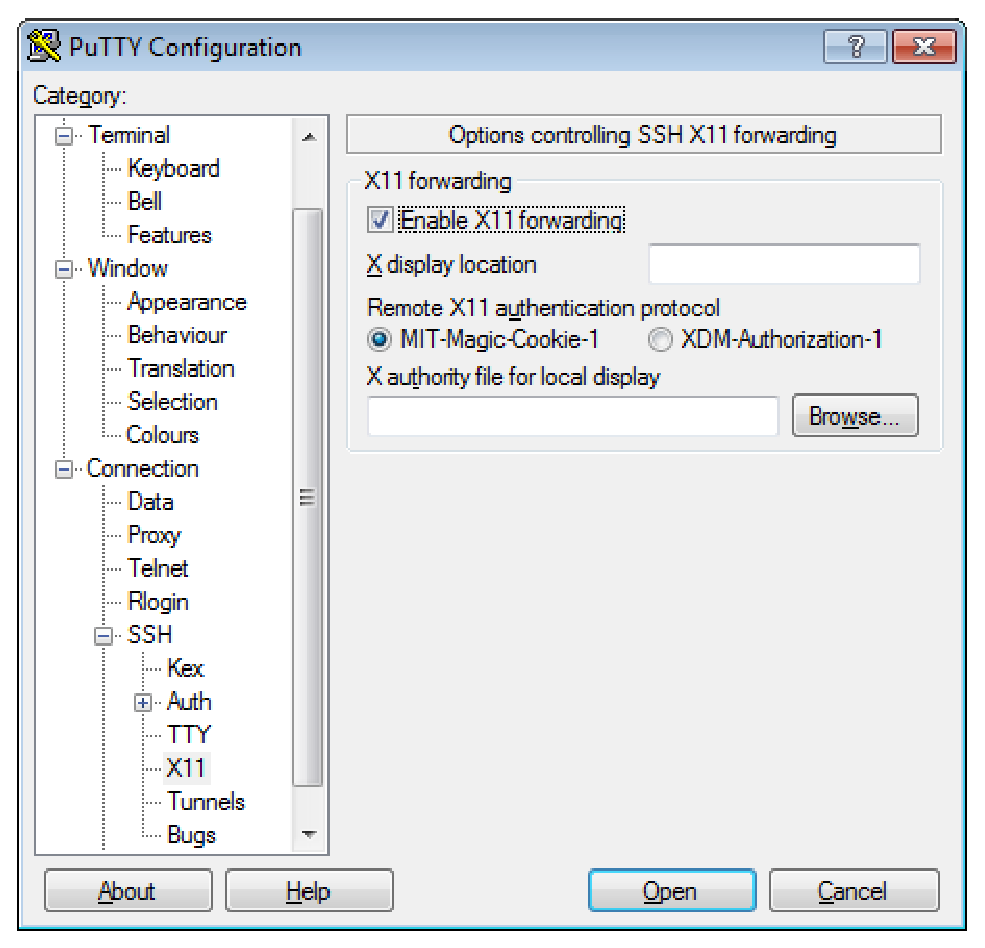
\includegraphics[width=0.6\textwidth]{./../eps/putty-x-forwarding.eps}
  \caption{Configure PuTTY for X forwarding over SSH.}
  \label{fig:putty-x-forwarding}
\end{figure}

At the prompt, you can quickly test whether the remote system is connected to your local X server by typing:
\begin{lstlisting}[style=basic,style=bash]
jspaaks@login4:~$ echo $DISPLAY
\end{lstlisting}\index{Linux commands!echo \char`\$
DISPLAY@\texttt{echo \$DISPLAY}}%Linux commands!echo DISPLAY@\texttt{echo DISPLAY}
which should result in a message like this (the numbers could be different):
\begin{lstlisting}[style=basic,style=bash]
localhost:10.0
\end{lstlisting}
If the connection was unsuccessful, the shell returns an empty message.

Start Octave in silent mode by:
\begin{lstlisting}[style=basic,style=bash]
jspaaks@login4:~$ octave --silent
octave:1> 
\end{lstlisting}
and then run the \lstinline[style=bashinline]{peaks(30)} function.
\begin{lstlisting}[style=basic,style=bash]
octave:1> peaks(30)
octave:2>
\end{lstlisting}
After a few moments (depending on the bandwidth of your connection to LISA), it will show you Fig.~\ref{fig:octave-peaks-x-forwarding}.
\begin{figure}[!htb]
  \centering
    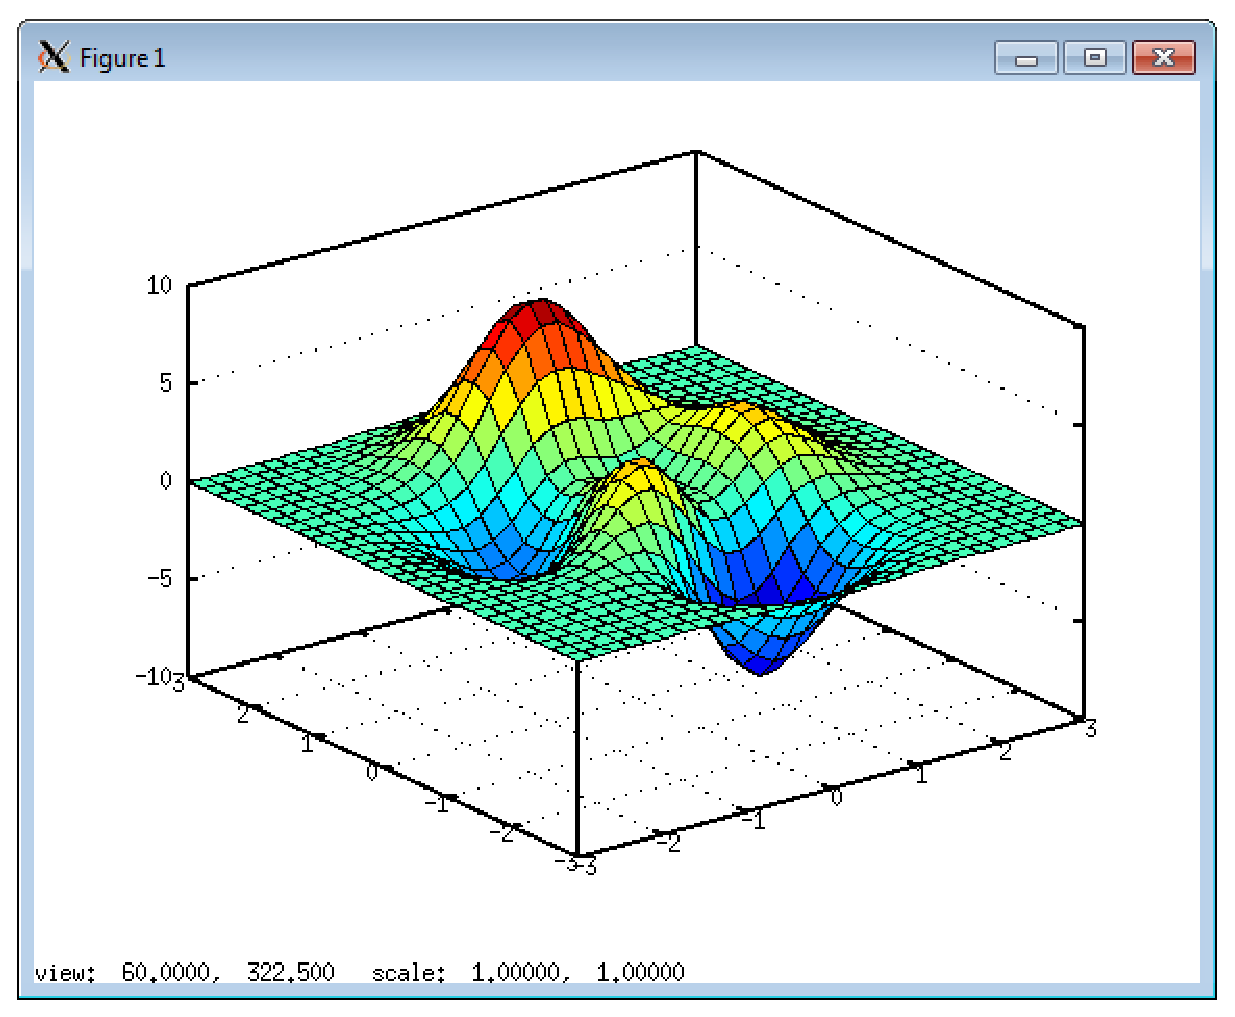
\includegraphics[width=0.6\textwidth]{./../eps/octave-peaks-x-forwarding.eps}
  \caption{After Octave generated this \lstinline[style=bashinline]{peaks(30)} figure remotely, the remote system sent it to the local machine over SSH where it was displayed with Xming.}
  \label{fig:octave-peaks-x-forwarding}
\end{figure}


\needspace{4em}
Let's see if we can do the same thing in MATLAB:
\begin{lstlisting}[style=basic,style=bash]
octave:2> exit

jspaaks@login4:~$ matlab
-bash: matlab: command not found
\end{lstlisting}
The reason this does not work is that MATLAB is only used by some users, therefore it is not available by default\footnote{In fact, you must be a member of the `MATLAB users group' that exist on LISA. Any of LISA's administrators can add you to this group, but it usually involves some administration.}. However, it's easy enough to make MATLAB available, like so:  
\begin{lstlisting}[style=basic,style=bash]
jspaaks@login4:~$ module load matlab
jspaaks@login4:~$ matlab 
\end{lstlisting}
It is considered good practice to \lstinline[style=bashinline]{unload} MATLAB once you are done with it:
\begin{lstlisting}[style=basic,style=bash]
jspaaks@login4:~$ module unload matlab
\end{lstlisting}
This frees up one of the MATLAB licenses, such that other users may use it. There are currently enough MATLAB licenses to run 32 instances of MATLAB simultaneously; however, some of the toolboxes require a separate license. For some toolboxes there are only 3 licenses available, so if your program happens to use one of those, you can only use 3 MATLAB instances simultaneously. 

If you are just using the MATLAB licenses to run your programs on LISA, as opposed to doing development work, you can (legally) circumvent licensing problems by compiling your m-code, and running the compiled code with the \textit{MATLAB Compiler Runtime}\index{MATLAB Compiler Runtime} or \textit{MCR}\index{MCR}. The MCR can be loaded in a similar fashion as the full MATLAB suite:
\begin{lstlisting}[style=basic,style=bash]
jspaaks@login4:~$ module load mcr
\end{lstlisting}
%For more information on compiling code, this is a good starting point: \burl{https://grid.sara.nl/wiki/index.php/Using_the_Grid/Lsg-matlab}

\begin{figure}[!htb]
  \centering
    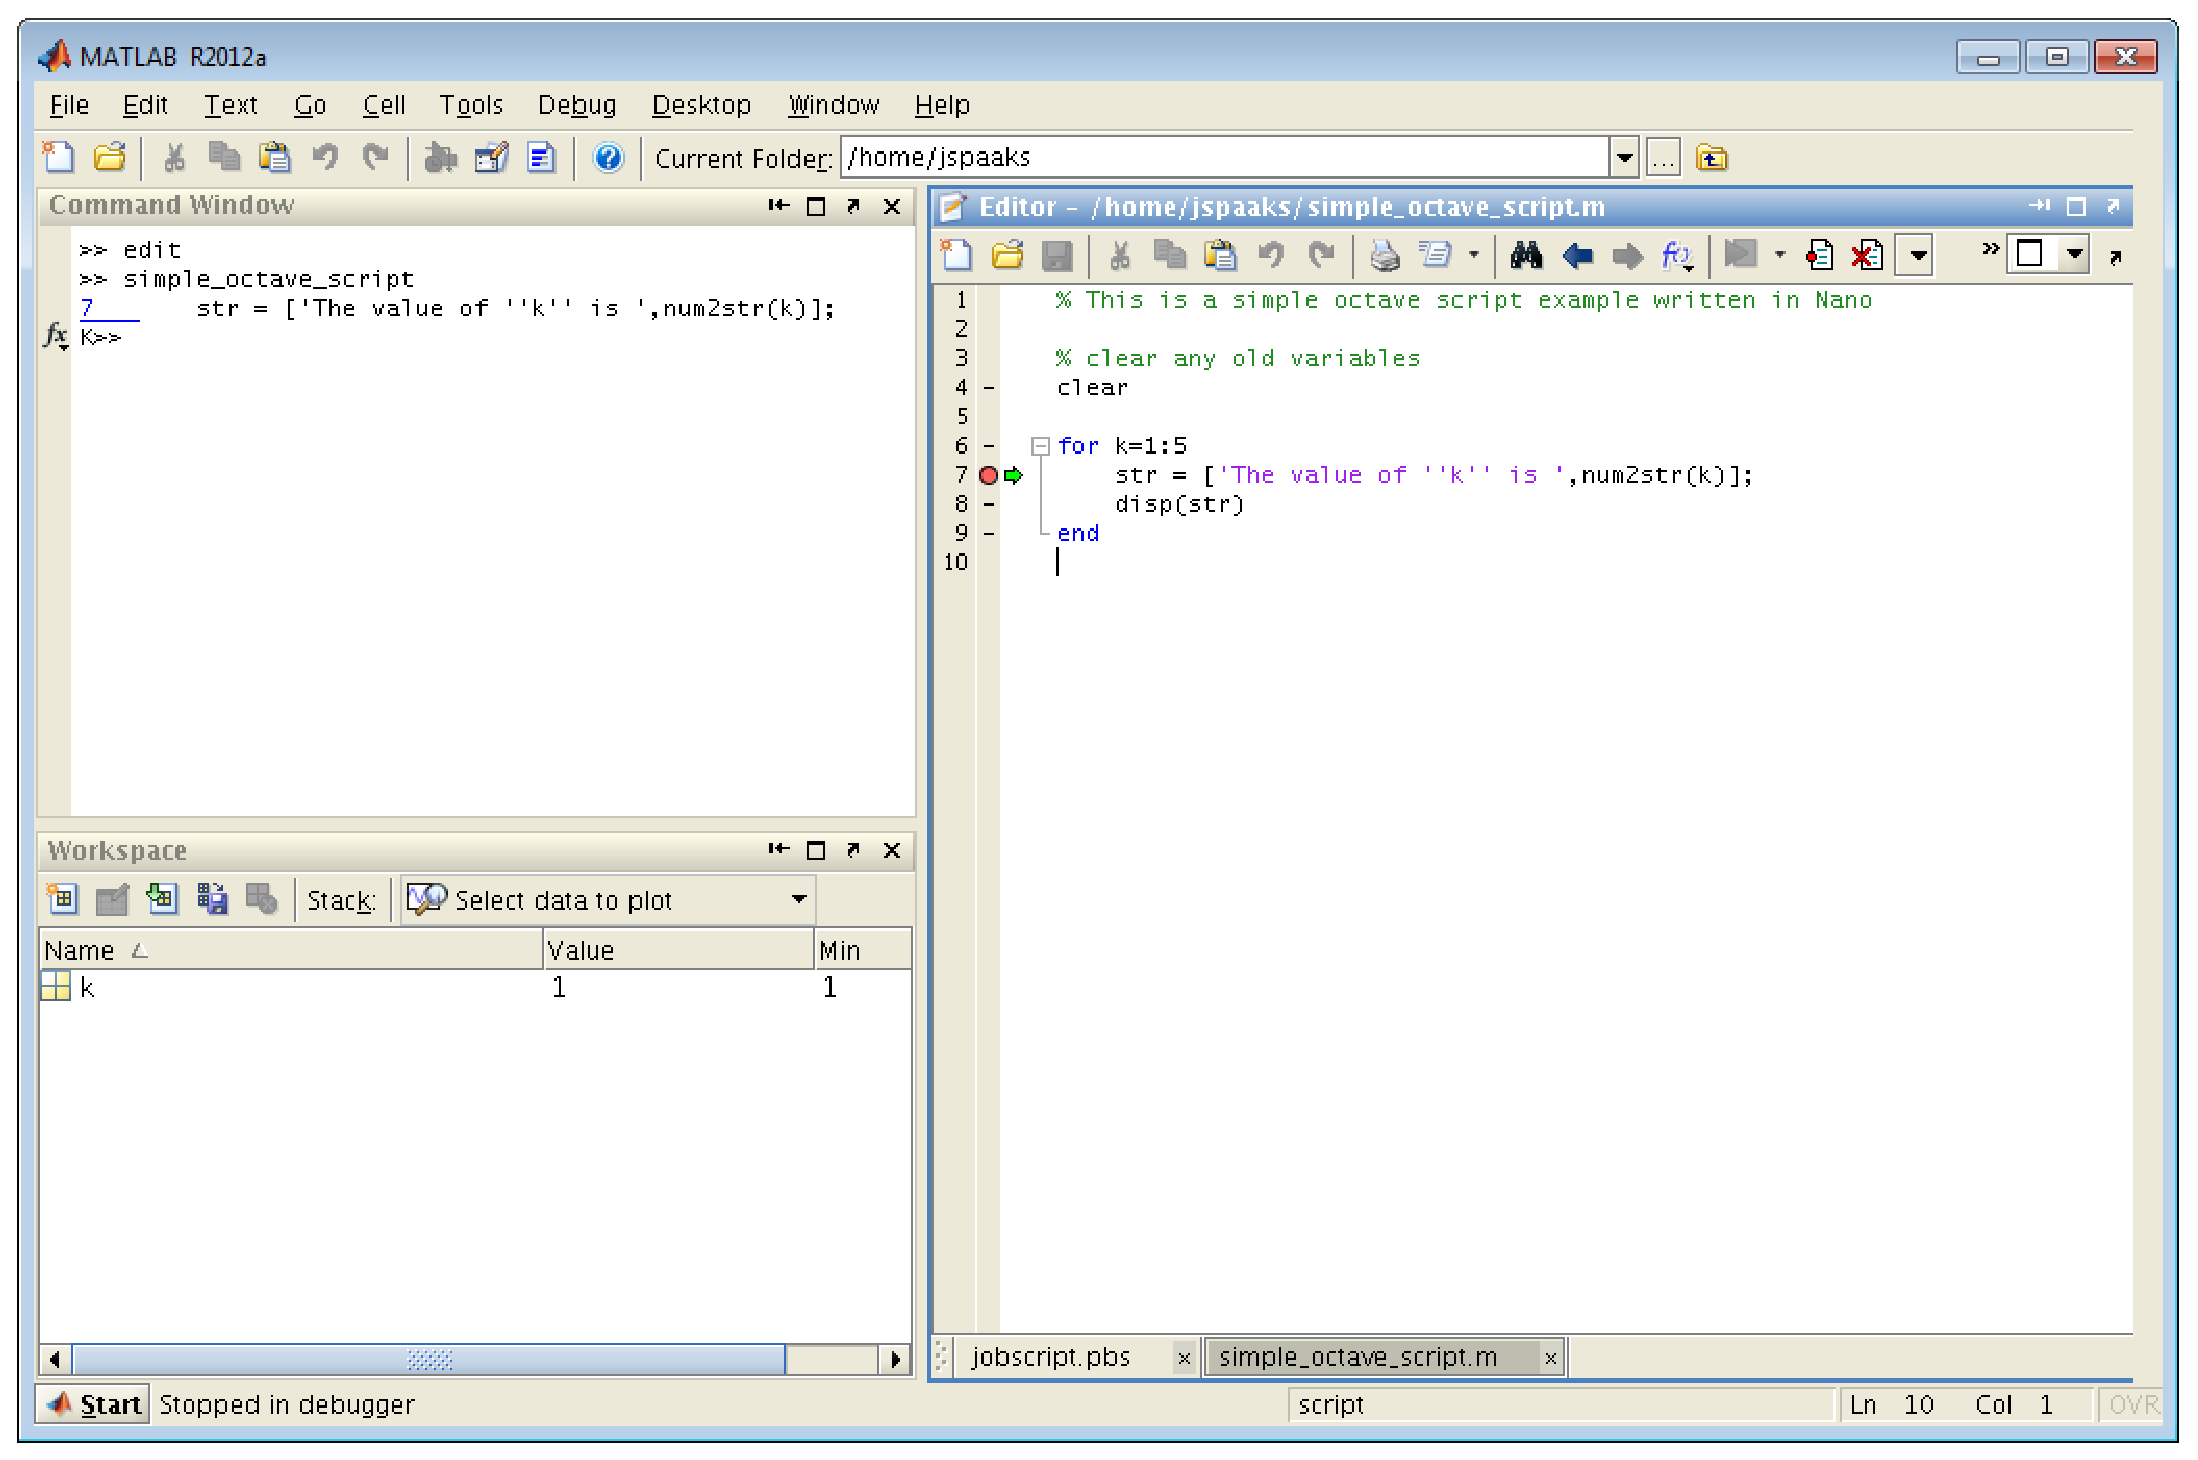
\includegraphics[width=0.9\textwidth]{./../eps/matlab-remote-debugging.eps}
  \caption{Even MATLAB's debugging capabilities can be used remotely!}
  \label{fig:matlab-remote-debugging}
\end{figure}


